%% TopoGuard: Adaptive Topology Orchestration for Risk-Sensitive Decision
%% under Hard Constraints and Multimodal Uncertainty
%% Submitted to ACM Transactions on Multimedia Computing, Communications and Applications (TOMM)
%%
%% Commands for TeXCount
%TC:macro \cite [option:text,text]
%TC:macro \citep [option:text,text]
%TC:macro \citet [option:text,text]
%TC:envir table 0 1
%TC:envir table* 0 1
%TC:envir tabular [ignore] word
%TC:envir displaymath 0 word
%TC:envir math 0 word
%TC:envir comment 0 0
%%
\documentclass[manuscript,review,anonymous]{acmart}

\usepackage{graphicx}
\usepackage{amsmath,amsfonts}
\usepackage{booktabs}
\usepackage{algorithm}
\usepackage{algpseudocode}
\setlength{\headheight}{20.5pt}
\addtolength{\topmargin}{-7.5pt}

\setcopyright{none}
\settopmatter{printacmref=true}
\renewcommand\footnotetextcopyrightpermission[1]{}


%%
%% \BibTeX command to typeset BibTeX logo in the docs
\AtBeginDocument{%
  \providecommand\BibTeX{{%
    Bib\TeX}}}


%%
%% end of the preamble, start of the body of the document source.
\begin{document}

%%
%% The "title" command has an optional parameter,
%% allowing the author to define a "short title" to be used in page headers.
\title{TopoGuard: Adaptive Topology Orchestration for Risk-Sensitive Decision Systems under Hard Constraints and Multimodal Uncertainty}



%%
%% The abstract is a short summary of the work to be presented in the
%% article.
\begin{abstract}
Risk-sensitive decision systems, such as storm-surge warning and emergency response, increasingly rely on multi-stage collaboration among heterogeneous modules and multimodal evidence. Such systems face a dual challenge: multimodal uncertainty, such as noisy sensors or conflicting weather patterns, can destabilize evidence reliability, while hard operational constraints, such as safety thresholds, strict time windows, and mandatory human oversight, make unconstrained trial-and-error or full online replanning difficult to justify. Fixed pipelines are easy to deploy but brittle across structurally diverse task instances. We propose \textbf{TopoGuard}, a profile-guided adaptive topology orchestration framework designed to construct feasible and reliable execution workflows under quality--cost--latency constraints. Instead of exhaustive online search, TopoGuard maintains task-conditional quality--cost--latency profiles for candidate workflow templates and executor assignments, uses constrained Pareto selection to generate an initial topology aligned with the current task difficulty and operational constraints, and records execution feedback for profile update. During execution, evaluator modules monitor intermediate output quality and trigger bounded local repair when failures occur; the repair procedure upgrades only affected stages rather than replanning the entire workflow. Experiments on a water-conservancy digital-twin platform show that TopoGuard reaches a favorable quality--cost--latency operating point compared with fixed workflows, executor-only routing, and single-objective selection baselines. Component and difficulty-wise analyses further suggest that topology-level adaptation is most useful when task instances differ in structural requirements, while bounded local repair provides additional recovery when intermediate execution quality degrades.
\end{abstract}

%%
%% The code below is generated by the tool at http://dl.acm.org/ccs.cfm.
%% Please copy and paste the code instead of the example below.
%%
\begin{CCSXML}
<ccs2012>
   <concept>
       <concept_id>10002951.10003227.10003241</concept_id>
       <concept_desc>Information systems~Decision support systems</concept_desc>
       <concept_significance>500</concept_significance>
   </concept>
   <concept>
       <concept_id>10002951.10003227.10003251</concept_id>
       <concept_desc>Information systems~Multimedia information systems</concept_desc>
       <concept_significance>500</concept_significance>
   </concept>
   <concept>
       <concept_id>10010147.10010178</concept_id>
       <concept_desc>Computing methodologies~Artificial intelligence</concept_desc>
       <concept_significance>300</concept_significance>
   </concept>
   <concept>
       <concept_id>10010147.10010178.10010199</concept_id>
       <concept_desc>Computing methodologies~Planning and scheduling</concept_desc>
       <concept_significance>300</concept_significance>
   </concept>
</ccs2012>
\end{CCSXML}

\ccsdesc[500]{Information systems~Decision support systems}
\ccsdesc[500]{Information systems~Multimedia information systems}
\ccsdesc[300]{Computing methodologies~Artificial intelligence}
\ccsdesc[300]{Computing methodologies~Planning and scheduling}

%%
%% Keywords. The author(s) should pick words that accurately describe
%% the work being presented. Separate the keywords with commas.
\keywords{Multimedia Systems, Topology Orchestration, Multimodal Decision Support, Workflow Optimization, Local Graph Repair, Digital Twin}
%% A "teaser" image appears between the author and affiliation
%% information and the body of the document, and typically spans the
%% page.

\begin{teaserfigure}
\centering
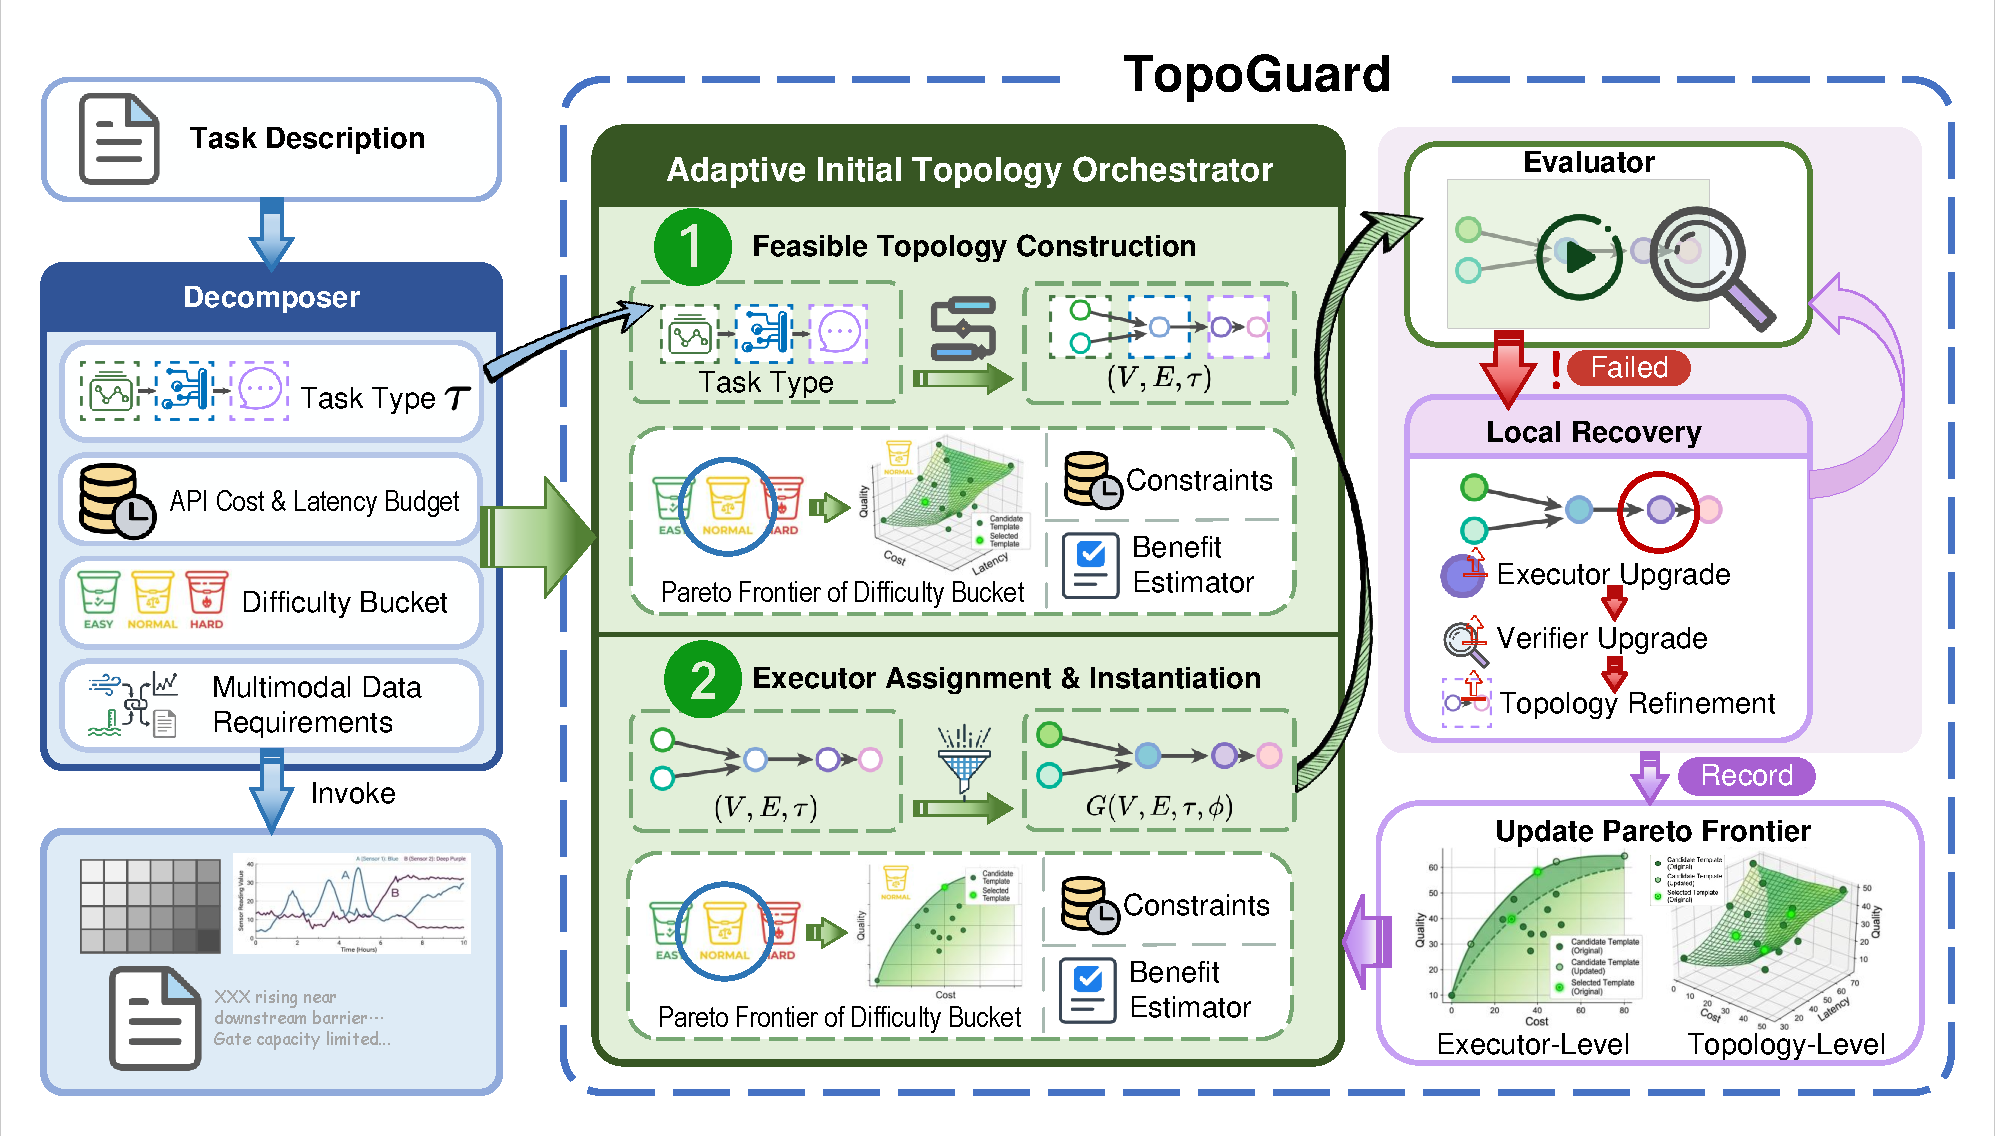
\includegraphics[width=\linewidth]{figures/fig2_v2.pdf}
\caption{Overview of the TopoGuard framework. The system takes a task description, resource constraints, and multimodal inputs, constructs an initial executable workflow through topology-level and executor-level Pareto-guided selection, monitors execution with an evaluator, and performs bounded local recovery through executor upgrade, verifier upgrade, or topology refinement when failures occur.}
\Description{Overview of the TopoGuard framework. The system takes a task description, resource constraints, and multimodal inputs, constructs an initial executable workflow through topology-level and executor-level Pareto-guided selection, monitors execution with an evaluator, and performs bounded local recovery through executor upgrade, verifier upgrade, or topology refinement when failures occur.}
\label{fig:framework}
\end{teaserfigure}

% \received{20 February 2007}
% \received[revised]{12 March 2009}
% \received[accepted]{5 June 2009}

%%
%% This command processes the author and affiliation and title
%% information and builds the first part of the formatted document.
\maketitle

\section{Introduction}
Modern multimodal intelligent systems are increasingly used for decision support in risk-sensitive domains such as hydrological analysis, infrastructure monitoring, and emergency response \cite{algiriyage2022multi,cheng2023review,inyang2025digital,tomczak2024development}. In these settings, task completion typically requires the coordinated use of heterogeneous functional modules, including data retrieval, numerical computation, reasoning, and verification \cite{zhang2024mm,huang2024understanding,zhai2025survey}. System effectiveness therefore depends not only on individual executors, but also on how they are organized into an executable collaboration topology.

However, such systems face a dual challenge: multimodal uncertainty (e.g., noisy sensors or conflicting weather patterns) destabilizes evidence reliability, while hard constraints (e.g., safety thresholds, strict time windows, and mandatory human oversight) prohibit unconstrained online exploration. Many deployed systems still rely on manually designed workflows or fixed model-selection rules where functional nodes and execution order are predetermined \cite{zeng2023flowmind,li2024autoflow,zhang2024aflow,fan2024workflowllm}. Such designs are easy to deploy but brittle in uncertain environments: different task instances require different processing structures; intermediate outputs may fail; and execution must satisfy constraints on quality, cost, and latency. A workflow that performs well for one instance may become expensive, slow, or ineffective for another, especially in risk-sensitive applications where local failures can propagate into unreliable downstream decisions \cite{tang2016emergency}. This issue is further amplified in multimodal settings with missing or unreliable modalities \cite{wu2024mlmmsurvey,lan2025robust,reza2024robust,liaqat2025chameleon}. In these settings, trial-and-error exploration is often infeasible because failed executions may consume scarce response time or violate operational safeguards.

Existing approaches attempt to improve adaptability through tool use, reasoning-action loops, and parallel function scheduling \cite{schick2023toolformer,yao2023react,kim2024llm}. However, the core decision is not only which executor to use, but also which functional nodes should be activated, how they should be connected, and how the execution graph should be adjusted when failures occur. In other words, the decision variable is the workflow topology itself. Recent work on LLM planning and workflow generation highlights structured execution organization, but mainly focuses on planning quality rather than topology adaptation under runtime constraints \cite{huang2024understanding,zhai2025survey,li2024autoflow,zhang2024aflow,fan2024workflowllm}. We therefore formulate the problem as \emph{adaptive topology orchestration} under hard constraints and multimodal uncertainty.

To address this problem, we propose \textbf{TopoGuard}, an adaptive topology orchestration framework for risk-sensitive decision systems. TopoGuard treats workflow execution as a closed-loop decision process over structured graphs. It maintains task-conditional quality--cost--latency profiles for candidate workflow templates and executor assignments. Based on these profiles, TopoGuard performs constrained Pareto-based selection to obtain an initial executable graph aligned with the current task difficulty and operational constraints. During execution, evaluator modules monitor intermediate outputs and detect local failures or reliability risks. Instead of triggering global replanning, TopoGuard performs bounded local graph repair that upgrades only affected stages while preserving reusable upstream computation.

A central observation motivating this work is that robust multimodal decision systems may benefit from choosing and maintaining better \emph{collaboration topologies}, rather than focusing solely on component selection. Topology-level adaptation allows the execution graph to adjust to task requirements, resource constraints, and runtime uncertainty, which is relevant for balancing effectiveness, efficiency, and reliability in risk-sensitive environments.

We evaluate TopoGuard on representative tasks involving heterogeneous executors and structured workflow operators. Experimental results show that TopoGuard reaches a favorable quality--cost--latency operating point compared with fixed workflows, executor-only routing, and single-objective baselines. Additional analyses indicate that bounded local repair provides useful recovery when intermediate execution quality degrades, and that topology-level adaptation is especially relevant when task instances differ in structural requirements.

\noindent\textbf{The main contributions of this paper are summarized as follows:}
\begin{itemize}
    \item \textbf{Problem Formulation.} We formulate adaptive workflow execution in risk-sensitive multimodal systems as an adaptive topology orchestration problem under hard constraints and multimodal uncertainty.
    \item \textbf{TopoGuard Framework.} We propose \textbf{TopoGuard}, a feasibility-aware topology orchestration framework that integrates offline performance profiling, constrained Pareto-based initial topology selection, and evaluator-triggered bounded local repair.
    \item \textbf{Empirical Validation.} We evaluate TopoGuard on a water-conservancy digital-twin platform and show that it achieves a favorable quality--cost--latency operating point compared with fixed, routing-only, and single-objective alternatives. Component analyses further indicate that topology selection, executor adaptation, and local repair contribute complementary benefits.
\end{itemize}

\section{Related Work}
\label{sec:related_work}

\subsection{Multimedia Decision Support and Digital Twins in High-Stakes Domains}

Multimedia systems are increasingly used beyond perception and retrieval, and have become part of decision-support pipelines in high-stakes settings such as emergency response, infrastructure monitoring, and hydrological analysis \cite{tang2016emergency,pathak2020hydroinformatics,yu2024warenet}. In water and infrastructure domains, recent digital-twin studies emphasize real-time monitoring, simulation, and decision support as core capabilities of intelligent management systems \cite{li2024intelligentwater,ge2025urbanflooddt}. These systems typically integrate heterogeneous observations, simulation outputs, and operational knowledge, but their execution logic is often implemented as manually designed pipelines or domain-specific control flows. Our work is related to this line of research in that it also targets decision support under multimodal inputs and operational constraints. The difference is that we focus on \emph{how} the execution structure should be selected and adjusted at runtime when task requirements, resource limits, and intermediate reliability vary across instances.

\subsection{Multimodal Uncertainty and Missing-Modality Robustness}

A large body of multimodal research studies robustness under missing, noisy, or unreliable inputs \cite{lan2025robust,wu2024mlmmsurvey}. This literature is directly relevant because real-world decision systems often operate with partial observability, degraded sensors, or cross-source inconsistency. Existing methods mainly improve robustness within a fixed model architecture or a fixed processing pipeline, for example through missing-modality learning, representation completion, or robust fusion. By contrast, we examine a different question: when evidence quality changes, should the system still use the same execution structure, or should it switch to a different workflow topology with additional verification or recovery stages? In this sense, our work complements model-level robustness methods by addressing structure-level adaptation.

\subsection{Workflow and Agent Orchestration}

Recent work on LLM-based agents has highlighted the value of structured execution rather than single-shot prompting. ReAct and Tree of Thoughts illustrate how intermediate reasoning and tool interaction can improve complex task solving \cite{yao2023react,yao2023tot}. More recent workflow-oriented approaches explicitly treat agent execution as a graph or workflow construction problem. For example, AFlow formulates agentic workflow generation as search over code-represented workflows and optimizes node-edge structure automatically \cite{zhang2024aflow}. These studies show that execution structure matters, but they primarily focus on producing strong workflows or better reasoning performance. Our setting is different in two respects: we consider hard deployment constraints on cost and latency during selection, and we explicitly model bounded local repair after execution has started.

\subsection{Cost-Aware Routing, Cascading, and Runtime Recovery}

Another closely related line of research studies cost-aware model selection and cascading. FrugalGPT shows that routing or cascading across models can reduce inference cost while maintaining strong task performance \cite{chen2023frugalgpt}. Subsequent work further unifies routing and cascading and highlights the importance of quality estimation for cost-performance trade-offs \cite{dekoninck2024routing}. These methods are relevant because they also optimize quality under budget constraints, but they usually treat the decision variable as \emph{which model} to call for a given query. Our work instead treats the workflow topology itself as the decision variable, jointly considering node activation, graph structure, executor assignment, and local repair.

Our repair component is also related to the broader literature on workflow exception handling and adaptive failure recovery. Prior research in workflow systems and service composition has studied exception handling, ad-hoc recovery, and adaptive failure handling for composite processes \cite{chiu2001exception,sato2010adaff}. Those studies motivate the importance of runtime recovery, but they are generally not formulated around modern multimodal agent workflows or multi-objective quality-cost-latency trade-offs. We build on the same general intuition that failures should be handled locally when possible, while instantiating it in a profile-guided orchestration framework for multimodal decision systems.




% Overleaf-ready English method section for direct paste.
% Suggested packages in your preamble:
% \usepackage{amsmath,amssymb,amsfonts}
% \usepackage{algorithm}
% \usepackage{algpseudocode}





\section{Method}
\label{sec:method}

\subsection{Problem Setup}

We consider adaptive orchestration for multi-stage decision tasks. For an input task $X$, the system must choose (i) a workflow structure, (ii) executor assignments for the nodes in that structure, and (iii) a limited set of repair actions if execution quality falls below a threshold.

The framework has two coupled stages: initial topology selection under hard quality--cost--latency constraints, followed by bounded local repair when intermediate failures are detected. Because the workflow-graph space is combinatorial, direct search is impractical; we therefore use a hierarchical selection procedure together with minimal-change local repair.

\subsection{Initial Topology Selection under Hard Constraints}
\label{sec:init_objective}

We first formulate the construction of the initial executable workflow as a constrained topology selection problem.
Given an input task $X$, the policy $\pi$ selects an initial workflow graph $G_{\pi}(X)$ from the candidate graph space.
The objective is to maximize utility under hard structural and resource constraints:
\begin{equation}
\pi^\star
=
\arg\max_{\pi\in\Pi}
\;\mathbb{E}_{X\sim D}\big[Q(G_{\pi}(X),X)\big],
\label{eq:init_obj}
\end{equation}
subject to
\begin{equation}
\begin{aligned}
&G_{\pi}(X)\in\mathcal{G}_{\mathrm{DAG}},\\
&C(G_{\pi}(X),X)\le B(X),\\
&L(G_{\pi}(X),X)\le \Delta(X).
\end{aligned}
\label{eq:init_constraints}
\end{equation}

Here, $\mathcal{G}_{\mathrm{DAG}}$ denotes the space of valid directed acyclic workflow graphs,
$B(X)$ is the task-specific budget constraint, and $\Delta(X)$ is the latency constraint.
This stage determines only the \emph{initial} executable topology; repair actions during execution are formulated separately in Section~\ref{sec:repair}.

To compare quality, cost, and latency on a comparable scale, we use a normalized utility:
\begin{equation}
Q(G,X)=\alpha\,S_{\mathrm{norm}}(G,X)-\beta\,C_{\mathrm{norm}}(G,X)-\gamma\,L_{\mathrm{norm}}(G,X),
\label{eq:utility}
\end{equation}
where $\alpha,\beta,\gamma\ge 0$ and $\alpha+\beta+\gamma=1$.
In our implementation, quality is normalized as
\begin{equation}
S_{\mathrm{norm}}(G,X)=\frac{S(G,X)}{S_{\mathrm{scale}}},
\label{eq:s_norm}
\end{equation}
and cost and latency use the normalized profile values $C_{\mathrm{norm}}$ and $L_{\mathrm{norm}}$ for candidate comparison.
Unless otherwise specified, we use $\alpha=0.65$, $\beta=0.25$, $\gamma=0.10$, and $S_{\mathrm{scale}}=1.5$.
Pareto frontiers are used only for candidate pruning before the final utility-based selection.

\subsection{Workflow Representation}

A workflow is represented as a directed graph
\begin{equation}
G=(V,E,\tau,\rho,\phi),
\end{equation}
where $V$ is the node set, $E\subseteq V\times V$ is the directed edge set, $\tau(v)$ is node role type, $\rho(v)$ is executor function type, and $\phi(v)$ is runtime configuration. DAG topology is enforced by a topological order $\operatorname{ord}:V\rightarrow\{1,\dots,|V|\}$ such that
\begin{equation}
(u,v)\in E\Rightarrow \operatorname{ord}(u)<\operatorname{ord}(v).
\end{equation}

Task context is encoded into a discrete difficulty level $b \in \{\text{easy}, \text{medium}, \text{hard}\}$, estimated from task features such as query length, domain complexity, and retrieval scope. The resulting difficulty level is used to condition both template retrieval and executor candidate selection.

In the current implementation, topology adaptation is instantiated as selection over a finite template library rather than arbitrary DAG generation. This design is intentional for risk-sensitive deployments, where candidate structures must be auditable, profileable, and feasible under operational constraints. The framework itself is not limited to the four templates used in our experiments; larger template libraries, including parallel or hierarchical structures, can be incorporated once sufficient profile data are available.

\subsection{Difficulty-Aware Hierarchical Initialization}

Given task $X$ and difficulty level $b$, initialization is decomposed into two levels:
\begin{equation}
T_0=\pi_{\text{init}}^{T}(X,b),
\qquad
\Phi_0=\pi_{\text{init}}^{N}(X,b,T_0),
\qquad
G_0=(T_0,\Phi_0).
\end{equation}

At the template level, we first perform Pareto pruning over candidate topologies:
\begin{equation}
\mathcal{P}_T=\text{Pareto}_{\max S,\min C,\min L}(\mathcal{T}(X,b)),
\end{equation}
and then select the feasible template with highest proxy utility:
\begin{equation}
T_0=\arg\max_{T\in\mathcal{P}_T^{\text{feasible}}}\widehat{Q}_T(T;X,b).
\end{equation}

At the node level, each executor node retrieves a difficulty-conditioned candidate pool,
\begin{equation}
\mathcal{A}_v(b,\rho(v)),
\qquad
\mathcal{P}_N(v)=\text{Pareto}_{\max S,\min C}(\mathcal{A}_v(b,\rho(v))),
\end{equation}
and selects the feasible candidate with maximal utility:
\begin{equation}
Q_N(a;v,X,b)=\alpha_N S(a;v,X,b)-\beta_N C(a;v,X,b),
\end{equation}
\begin{equation}
\phi(v)=\arg\max_{a\in\mathcal{P}_N^{\text{feasible}}(v)}Q_N(a;v,X,b).
\end{equation}

\subsection{Bounded Local Repair with Edit-Loss}
\label{sec:repair}

After the initial workflow $G_0$ has been selected and instantiated, execution proceeds in a closed loop.
When the evaluator detects that an intermediate result fails the pass condition, TopoGuard does not re-optimize the whole graph from scratch.
Instead, it performs bounded local repair around the affected region.

At execution step $t$, let $G_t$ denote the current workflow graph and $s_t$ the local execution state.
A repair action is selected as
\begin{equation}
a_t=\pi_{\mathrm{repair}}(s_t),
\qquad
G_{t+1}=\mathcal{T}_{\mathrm{op}}(G_t,a_t),
\label{eq:repair_transition}
\end{equation}
where $\mathcal{T}_{\mathrm{op}}$ applies a local graph edit to the current workflow.

We consider three repair operators,
\begin{equation}
\mathcal{A}_t=\{A,B,C\},
\end{equation}
corresponding to topology/template upgrade, executor upgrade, and evaluator upgrade, respectively.
To discourage unnecessary large edits, we define the edit loss as
\begin{equation}
\mathcal{L}_{\mathrm{edit}}(a)
=
\lambda_n\Delta n(a)+\lambda_\phi\Delta\phi(a)+\lambda_e\Delta e(a),
\label{eq:edit_loss}
\end{equation}
where $\Delta n(a)$, $\Delta\phi(a)$, and $\Delta e(a)$ measure changes in nodes, executor assignments, and edges.
In our implementation, the weights are set to $\lambda_n=0.30$, $\lambda_\phi=0.25$, $\lambda_e=0.10$, and the overall penalty weight is $\lambda=0.20$.

The repair policy then solves a bounded local optimization problem:
\begin{equation}
a_t^\star
=
\arg\max_{a\in\mathcal{A}_t^{\mathrm{feasible}}}
\Big(
Q(G_{t+1}(a),X)-\lambda\,\mathcal{L}_{\mathrm{edit}}(a)
\Big),
\label{eq:repair_obj}
\end{equation}
where the feasible repair set is
\begin{equation}
\mathcal{A}_t^{\mathrm{feasible}}
=
\{a\in\mathcal{A}_t \mid S(G_{t+1}(a),X)\ge\tau_{\mathrm{pass}}\}.
\label{eq:repair_feasible}
\end{equation}
Here $\tau_{\mathrm{pass}}=0.5141$ is the data-driven repair trigger threshold (the 25th percentile of realized quality scores across training episodes), which is computed once from training data and held fixed at evaluation time.

This formulation separates repair from initial topology selection:
the initial stage chooses a globally feasible workflow under hard constraints, whereas repair performs \emph{local correction} aimed at restoring execution quality without global replanning.

\begin{algorithm}[t]
\caption{TopoGuard Hierarchical Pareto Orchestration}
\label{alg:hpo}
\begin{algorithmic}[1]
\Require Task $X$, performance profile $\mathcal{P}$, budget $B$, latency bound $\Delta$, repair threshold $\tau_{\mathrm{pass}}$
\Ensure Final workflow $G^*$ and execution result
\State $b \gets \textsc{EstimateDifficulty}(X)$ \Comment{estimate task difficulty level}
\State $\mathcal{F}_T \gets \textsc{ParetoFilter}(\mathcal{P}, b, B, \Delta)$ \Comment{template-level Pareto pruning}
\State $T_0 \gets \arg\max_{T \in \mathcal{F}_T} \hat{Q}(T; X, b)$ \Comment{select highest-utility template}
\For{each $v \in V(T_0)$}
    \State $\mathcal{F}_v \gets \textsc{ParetoFilter}(\mathcal{P}, v, b, B)$ \Comment{node-level Pareto pruning}
    \State $\phi(v) \gets \arg\max_{a \in \mathcal{F}_v} Q_N(a; v, X, b)$ \Comment{select best executor}
\EndFor
\State Execute workflow $G_0 = (T_0, \Phi_0)$, obtain intermediate outputs $\{o_v\}$
\For{each $v \in V(T_0)$}
    \If{$\textsc{Evaluator}(o_v) < \tau_{\mathrm{pass}}$} \Comment{evaluator detects local failure}
        \State $\mathcal{A}^{\mathrm{feas}} \gets \{a \in \{A,B,C\} \mid S(G(a)) \ge \tau_{\mathrm{pass}}\}$
        \State $a^* \gets \arg\max_{a \in \mathcal{A}^{\mathrm{feas}}} \bigl(Q(G(a)) - \lambda\,\mathcal{L}_{\mathrm{edit}}(a)\bigr)$
        \State $G_0 \gets \mathcal{T}_{\mathrm{op}}(G_0, a^*)$ \Comment{apply bounded local repair}
    \EndIf
\EndFor
\State Update profile $\mathcal{P}$; \Return $G^* \gets G_0$
\end{algorithmic}
\end{algorithm}


\section{Experiments}
\label{sec:experiments}

We evaluate TopoGuard as a closed-loop topology orchestration framework. 
For each task instance, the system first selects an executable workflow under quality--cost--latency constraints and then monitors execution for possible local repair. 
The experiments are organized around the following questions:

\begin{itemize}
    \item \textbf{RQ1:} Can TopoGuard reach a favorable operating point among quality, cost, and latency?
    \item \textbf{RQ2:} Does local repair contribute substantively to the final system performance?
    \item \textbf{RQ3:} Do the observed advantages remain stable across task domains and different utility preferences?
    \item \textbf{RQ4:} Can bounded local repair recover quality when realized execution behavior deviates from the profiled expectation?
\end{itemize}

\subsection{Experimental Setup}
\label{subsec:exp_setup}



\paragraph{Platform and task domains.}
We conduct all experiments on a water-conservancy digital-twin platform and evaluate TopoGuard on two representative task domains: \textbf{Water QA} and \textbf{Storm Surge}. 
The primary benchmark, \textbf{Water QA}, is formulated as a multi-stage question answering task over hydrological knowledge. 
Different task instances may require different execution structures, such as retrieval, reasoning, computation, verification, and aggregation. 
Multimodal uncertainty is operationalized through the task difficulty dimension: easy, medium, and hard instances differ in query ambiguity, retrieval noise, and the reliability of intermediate outputs, which directly affects which topology and executor combination is appropriate. The auxiliary benchmark, \textbf{Storm Surge}, is used to examine whether the learned orchestration strategy can transfer to another decision domain without redesigning the core decision logic.

\begin{figure}[t]
    \centering
    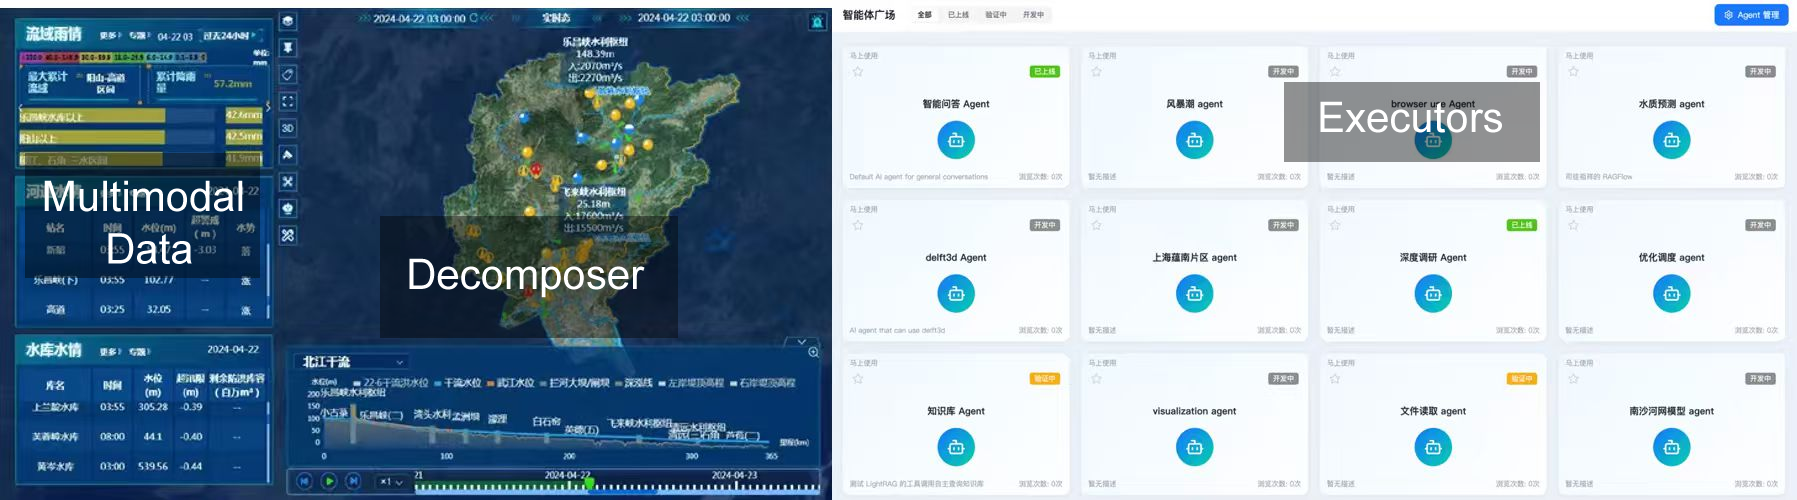
\includegraphics[width=0.88\textwidth]{figures/HW.png}
    \caption{The water-conservancy digital-twin agent platform used for evaluation. The platform integrates multimodal monitoring data, a task decomposition interface, and a pool of executable domain agents supporting heterogeneous workflow configurations.}
    \Description{Screenshot of the water-conservancy digital-twin agent platform showing task decomposition, agent pool, and monitoring interface.}
    \label{fig:platform}
\end{figure}

\paragraph{Data and evaluation protocol.}
For Water QA, we construct a benchmark containing training and test executions, which are further aggregated into historical performance profiles for candidate workflows and executors. 
For Storm Surge, we build an auxiliary transfer benchmark with heterogeneous execution choices and evaluate whether the same orchestration strategy can generalize across tasks. 
In both domains, the training split is used to estimate the expected quality, cost, and latency of candidate workflows, while all final results are reported on held-out test executions.

Given a test context, the system first queries historical profiles to estimate the expected triplet $(S,C,L)$ for each candidate topology or executor, applies hard constraint filtering, computes the feasible Pareto frontier, and then selects an execution plan according to the corresponding orchestration strategy.
For TopoGuard, the selected plan is further executed in a closed loop with evaluator monitoring and optional local repair.

Table~\ref{tab:benchmark_stats} summarizes the benchmark construction statistics. The Water QA benchmark comprises 17 models $\times$ 5 node types $\times$ 3 difficulty levels, yielding 163 non-empty profile entries (some combinations lack training coverage; notably, (retrieval, hard) has no valid candidates, affecting some test contexts). The Pareto frontier contains 24 feasible candidates, from which all strategies select. All profiles are estimated from training episodes on the same platform; no external data is used.

\begin{table}[t]
\centering
\caption{Benchmark construction statistics for the Water QA domain.}
\label{tab:benchmark_stats}
\small
\begin{tabular}{lr}
\toprule
\textbf{Item} & \textbf{Count / Value} \\
\midrule
Candidate models & 17 \\
Node types & 5 (retrieval, reasoning, computation, verification, aggregation) \\
Difficulty levels & 3 (easy, medium, hard) \\
Topology templates & 4 (direct, bad\_direct, ex+ver, ex+ver+agg) \\
Profile entries & 163 \\
Pareto frontier size & 24 \\
Training records & 1,467 \\
Test contexts (unique) & 255 \\
Test episodes (total) & 834 \\
Constraint budget $C_{\max}$ & 0.5 (log-normalized) \\
Latency budget $L_{\max}$ & 0.90 (log-normalized) \\
$Q$-score scale $S_{\text{scale}}$ & 1.5 \\
\bottomrule
\end{tabular}
\end{table}

\paragraph{Compared methods.}
We compare TopoGuard with six alternative orchestration strategies, organized by whether they select from the Pareto feasible candidate pool:

\textbf{Candidate-pool selection methods} (selecting from the 24 non-dominated Pareto candidates, pruned from 46 feasible candidates):
\begin{itemize}
    \item \textbf{TopoGuard (dual-layer adaptive):} performs Pareto pruning and utility-maximization selection at both the template level and the executor level, with bounded local repair. This is the full framework proposed in this paper.
    \item \textbf{LLM Router (executor-only adaptive):} selects the best executor by estimated quality within a fixed topology template (executor+verifier), without adapting workflow structure. Models the common model-routing approach and isolates the contribution of topology-level adaptation.
    \item \textbf{Random:} uniformly samples a candidate from the feasible Pareto frontier, serving as a no-adaptation baseline.
    \item \textbf{Best-Quality / Cheapest:} select the candidate with the highest estimated quality or the lowest estimated cost, serving as single-objective baselines.
\end{itemize}

\textbf{Fixed-pipeline methods} (not selecting from the candidate pool):
\begin{itemize}
    \item \textbf{Static Workflow:} fixes the topology to executor+verifier and the executor to kimi\_k2\_5. No Pareto screening, no adaptive topology selection, and no repair. This conservative non-adaptive pipeline serves as an alternative operating point for evaluating the quality-overhead trade-off.
    \item \textbf{FrugalGPT Cascade:} sorts executors by cost and selects the first meeting $S \geq 0.70$, without topology adaptation. Models the ``call cheap model first, escalate only if needed'' strategy.
\end{itemize}

This organization highlights the core innovation of TopoGuard---dual-layer adaptive topology selection---and provides controlled comparisons that isolate the contribution of each adaptive layer. The Static Workflow comparison evaluates whether the adaptive overhead is worthwhile in practice, rather than competing on a single metric.


\paragraph{Metrics.}
We report three primary metrics: \textbf{quality} $S\in[0,1]$, \textbf{cost} $C$ (USD), and \textbf{latency} $L$ (seconds).
Quality measures the final task-solving effectiveness of the selected workflow.
Cost is computed from actual execution expenses, and latency records the realized end-to-end execution delay.
Following the current implementation, cost and latency are log-normalized only for internal Pareto filtering, while all reported results use raw values for interpretability.

Note that the \textbf{violation rate (Viol\%)} is \emph{zero by construction} in our controlled selection experiment: all strategies select from a hard-filtered feasible set that excludes candidates violating the budget or latency constraints. This guarantees ex-ante feasibility for all methods, making Viol\% undifferentiated in this setting. The role of hard constraints in this experiment is therefore to \emph{shape the candidate pool}: tightening $C_{\max}$ removes expensive candidates and forces selection toward cheaper topologies, which changes the quality--cost operating point even when no violation occurs. Violation rate becomes meaningful only when estimated profiles mismatch actual execution conditions, as studied in the profile-drift experiment (Section~\ref{subsec:sensitivity}), where inflating estimated latency by 50\% shifts topology selection and reduces quality from $S=0.798$ to $S=0.770$ (Table~\ref{tab:drift_results}).

A related auxiliary metric is the \textbf{valid context rate}: the fraction of test contexts for which at least one feasible candidate exists in the profile (i.e., $N / N_{\text{total}}$ in the result tables). A context is \emph{invalid} if every candidate profile for that (node\_type, difficulty) pair violates either the budget constraint ($C > B$) or the latency constraint ($L > \Delta$). Context coverage directly reflects the feasibility of the candidate pool under given constraints; a higher valid context rate indicates broader operational coverage.

The valid context count $N$ varies across strategies. The primary source is missing profile coverage for the (retrieval, hard) pair, which causes Random ($N=244$) to fall below 255; all other strategies cover the full 255 contexts.

The internal selection metric $Q(G;X)=\alpha S_{\text{norm}}-\beta C_{\text{norm}}-\gamma L_{\text{norm}}$ is used solely for Pareto frontier ranking and candidate tie-breaking; it does not appear as a reported evaluation metric. $S_{\text{norm}}=S / S_{\text{scale}}$ normalizes quality to the same scale as $C_{\text{norm}}$ and $L_{\text{norm}}$, preventing quality from dominating the score purely due to scale differences. In our implementation, $(\alpha,\beta,\gamma)=(0.65,0.25,0.10)$ with $S_{\text{scale}}=1.5$, which balances quality prioritization with genuine cost-latency trade-offs on the Pareto frontier.

\subparagraph{Experiment protocol.}\label{subsubsec:exp_protocol}
Our experiments consist of two complementary evaluation protocols:
\textbf{(1) Shared-pool controlled comparison}: Random, Best-Quality, and Cheapest are evaluated as controlled selection baselines on the same learned profiles, selecting from the shared feasible candidate pool. This isolates the effect of the decision heuristic while holding the candidate space fixed.
\textbf{(2) Operating-point comparison}: TopoGuard and Static Workflow are evaluated on the same test contexts but represent different deployment philosophies (adaptive vs.\ fixed). They are not compared on a single metric; instead, the two are contrasted on their respective strengths: TopoGuard on quality and adaptive robustness, Static Workflow on cost-efficiency and simplicity.

\paragraph{Implementation details.}
The full TopoGuard pipeline consists of: 
(1) initial context analysis, 
(2) workflow-level candidate screening, 
(3) node-level executor selection, 
(4) execution and evaluator monitoring, and 
(5) bounded local repair. 
The repair operators are defined as three types: topology/template upgrade (operator A), executor upgrade (operator B), and evaluator upgrade (operator C). In the 500-round closed-loop evaluation, 451 of 675 execution contexts trigger repair (66.8\%), with operator C1 (cross-topology executor upgrade) accounting for 54.3\% of cases, operator B (executor upgrade) for 20.0\%, topology upgrade (operator A) for 21.5\%, and operator C2 for 4.2\%; full statistics are reported in Section~\ref{subsec:ablation_repair}.

\subsection{Main Results on Water QA}
\label{subsec:main_results}

\begin{figure}[t]
    \centering
    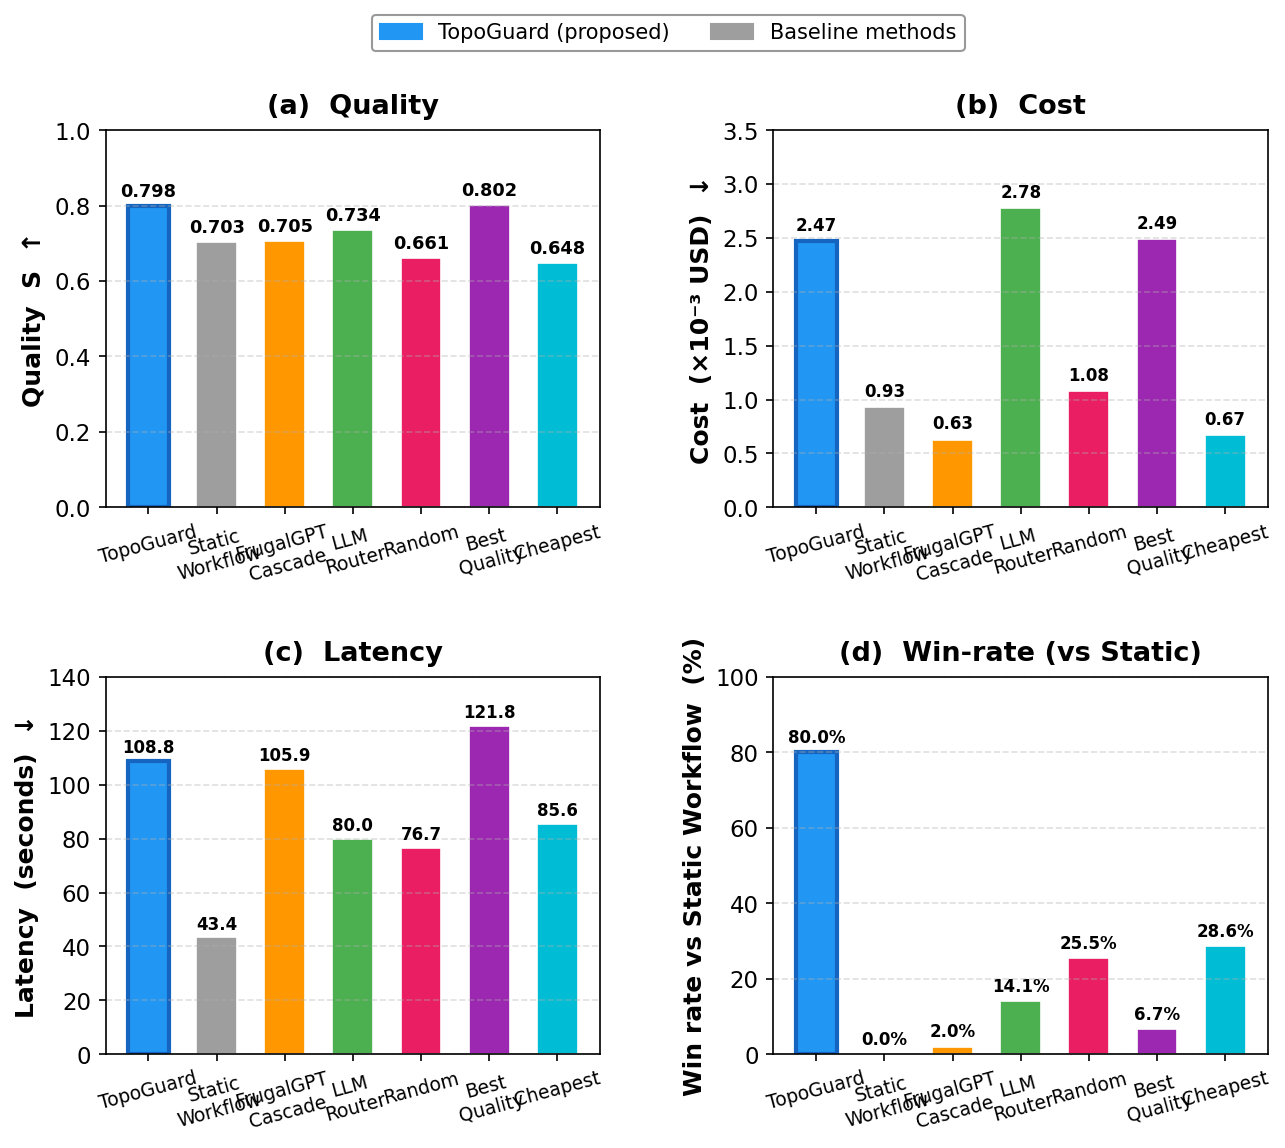
\includegraphics[width=0.96\textwidth]{figures/figA_2x2.png}
    \caption{Strategy comparison on Water QA (500 rounds, $N=255$ contexts). TopoGuard achieves a favorable quality--cost--latency operating point: quality within $\sim$1\% of Best-Quality, latency 11\% lower, while Static Workflow and FrugalGPT Cascade target the low-cost fixed-pipeline corner. See panels (a)--(d) for per-metric breakdown and win-rate analysis.}
    \Description{Bar charts comparing TopoGuard and baselines on Water QA across quality, cost, and latency.}
    \label{fig:strategy_comparison_2x2}
\end{figure}

We first examine \textbf{RQ1}, namely whether TopoGuard reaches a favorable quality--cost--latency operating point on the Water QA benchmark.

Table~\ref{tab:water_qa_main} reports the closed-loop results on 500 held-out test rounds (834 episodes in total). Valid context counts ($N$) differ across strategies because profile coverage is incomplete for the (retrieval, hard) pair: all strategies except Random cover the full 255 contexts, while Random covers $N=244$.

\textbf{TopoGuard (adaptive)} reaches $S=0.798$ through profile-guided topology selection with bounded repair. Best-Quality achieves $S=0.802$ at higher latency ($121.8$\,s vs.\ $108.8$\,s) and comparable cost ($2.49\times10^{-3}$ vs.\ $2.47\times10^{-3}$ USD), reflecting different operating points in the quality--cost--latency space. On paired per-context comparison against Static Workflow ($n=255$, 204 wins / 0 ties / 51 losses), TopoGuard leads with a mean advantage of $\Delta S=+0.095$ ($0.798$ vs.\ $0.703$).

\textbf{Marginal gain decomposition (F-3 analysis).} To rule out the confound that quality gains come from more compute, we regress $\Delta S = \beta_0 + \beta_1 \cdot \Delta C$ over the 255 paired contexts: $\beta_0=+0.0861$ (intercept), $\beta_1=+5.705$ (marginal return), with Cohen's $d=0.777$ (medium-large effect). The intercept term provides an estimate of the quality advantage not explained by additional cost, which we interpret as evidence that topology selection contributes substantially to the observed gain (approximately 90.7\% of the total quality advantage). This pattern is more consistent with topology-aware selection than with a simple increase in resource investment.

\textbf{Static Workflow (fixed)} represents a conservative baseline with the executor+verifier topology and kimi\_k2\_5 executor, without adaptive selection. It achieves lower quality ($S=0.703$) but also lower cost ($C=9.33\times10^{-4}$ USD) and latency ($L=43.4$\,s). The relevant practical question is whether the quality gain justifies the additional operational overhead.

\textbf{FrugalGPT Cascade} and \textbf{LLM Router} represent established baselines from the literature. FrugalGPT Cascade ($S=0.705$, $C=6.29\times10^{-4}$ USD, $L=105.9$\,s) escalates greedily through executors ordered by cost until a quality threshold is met, without any topology adaptation. LLM Router ($S=0.734$, $C=2.78\times10^{-3}$ USD, $L=80.0$\,s) selects the best executor within a fixed topology template, adapting only the model choice. The gap between LLM Router and TopoGuard ($\Delta S \approx +0.064$) isolates the contribution of topology-level adaptation (see Section~\ref{subsec:ablation_repair}).

\begin{figure*}[t]
    \centering
    
\includegraphics[width=0.96\textwidth]{figures/figB_paired_scatter.png}
    \Description{Left: per-context scatter plot of TopoGuard quality vs Static Workflow quality. Right: histogram of per-context quality advantage delta S.}
    \caption{Per-context paired comparison of TopoGuard vs Static Workflow ($n=255$). \textbf{Left:} each point is one test context; points above the diagonal indicate TopoGuard wins. TopoGuard wins in 204/255 contexts (80.0\%), ties in 0, and loses in 51. \textbf{Right:} distribution of per-context quality advantage $\Delta S = S_{\text{TopoGuard}} - S_{\text{Static}}$; mean $\Delta S = +0.095$.}
    \label{fig:paired_scatter}
\end{figure*}

\begin{figure*}[t]
    \centering
    
\includegraphics[width=0.96\textwidth]{figures/figC_cdf_advantage.png}
    \Description{CDF of per-context quality advantage delta S for TopoGuard vs Static Workflow (left) and TopoGuard vs Best-Quality (right).}
    \caption{Cumulative distribution of per-context quality advantage $\Delta S$. \textbf{Left:} TopoGuard vs Static Workflow --- distribution is right-shifted (mean $+0.095$, 204/255 contexts TopoGuard wins). \textbf{Right:} TopoGuard vs Best-Quality --- distribution is slightly left-shifted (mean $-0.004$, 17 wins / 221 ties / 17 losses); TopoGuard achieves comparable quality at lower latency and cost.}
    \label{fig:cdf_advantage}
\end{figure*}

\begin{table}[t]
\centering
\caption{Closed-loop topology orchestration results on Water QA (500 rounds, 834 test episodes). All strategies select from the hard-filtered feasible set (Viol\% = 0\% by construction). Best-Quality achieves the highest quality ($S=0.802$) at the cost of higher latency ($121.8$\,s vs.\ $108.8$\,s for TopoGuard); all other methods are lower in quality.}
\label{tab:water_qa_main}
\resizebox{0.98\linewidth}{!}{
\begin{tabular}{lccccc}
\toprule
\textbf{Method} & \textbf{Quality $S$ $\uparrow$} & \textbf{Cost ($\times 10^{-3}$ USD) $\downarrow$} & \textbf{Latency (s) $\downarrow$} & \textbf{N} \\
\midrule
TopoGuard                                     & \textbf{0.798} & 2.47      & 108.8 & 255 \\
Static Workflow                               & 0.703          & \textbf{0.933}    & \textbf{43.4} & 255 \\
FrugalGPT Cascade~\cite{chen2023frugalgpt}    & 0.705          & 0.629     & 105.9 & 255 \\
LLM Router~\cite{kim2024llm}                  & 0.734          & 2.78      & 80.0  & 255 \\
Random                                        & 0.661          & 1.08      & 76.7  & 244 \\
Best-Quality                                  & 0.802          & 2.49      & 121.8 & 255 \\
Cheapest                                      & 0.648          & 0.667     & 85.6  & 229 \\
\bottomrule
\end{tabular}}
\end{table}

\textbf{Difficulty-wise breakdown.} Table~\ref{tab:difficulty_breakdown} reports quality at each difficulty level for TopoGuard, Static Workflow, and LLM Router. TopoGuard's absolute quality decreases from easy ($S=0.921$) to hard ($S=0.668$), consistent with harder instances having noisier profiles and lower base quality. The advantage over Static Workflow grows with difficulty, from $+0.048$ on easy contexts to $+0.134$ on hard contexts, indicating that topology-level adaptation is especially useful compared with a fixed pipeline when tasks become structurally more demanding. The margin over LLM Router also grows with difficulty ($+0.071$ easy, $+0.039$ medium, $+0.082$ hard), suggesting that topology selection provides complementary benefit to executor routing across all difficulty levels.

\begin{table}[t]
\centering
\caption{Quality by difficulty level on Water QA ($n=85$ per level). TopoGuard's advantage over Static Workflow grows with task difficulty; the margin over LLM Router is positive across all levels.}
\label{tab:difficulty_breakdown}
\small
\begin{tabular}{lccc}
\toprule
\textbf{Method} & \textbf{Easy} & \textbf{Medium} & \textbf{Hard} \\
\midrule
TopoGuard        & \textbf{0.921} & \textbf{0.803} & \textbf{0.668} \\
LLM Router       & 0.850          & 0.764          & 0.587 \\
Static Workflow  & 0.873          & 0.701          & 0.534 \\
\midrule
$\Delta$ vs Static     & $+0.048$ & $+0.102$ & $+0.134 \\
$\Delta$ vs LLM Router & $+0.071$ & $+0.039$ & $+0.082 \\
\bottomrule
\end{tabular}
\end{table}
%     \centering
%     
\includegraphics[width=0.98\textwidth]{figures/figA_strategy_comparison.png}
%     \caption{Strategy comparison on Water QA. TopoGuard achieves a stronger overall balance across quality, cost, and latency than the alternative orchestration strategies.}
%     \label{fig:strategy_comparison_2x2}
% \end{figure*}




\subsection{Pareto Structure Analysis}
\label{subsec:pareto_analysis}

To further interpret the trade-off, we examine the per-context quality differences and their cumulative distributions.

Figure~\ref{fig:paired_scatter} shows the paired comparison between TopoGuard and Static Workflow at the context level. Points above the diagonal correspond to contexts in which TopoGuard achieves higher quality. The win rate is 204/255 (80.0\%), with a mean advantage of $\Delta S = +0.095$. This pattern suggests that the gain is spread across the majority of contexts.

Figure~\ref{fig:cdf_advantage} reports the cumulative distribution of $\Delta S$ for two pairwise comparisons. Relative to Static Workflow, the distribution is strongly shifted to the right, consistent with the large positive mean advantage. Relative to Best-Quality, the distribution is slightly shifted to the left (mean $\Delta S = -0.004$), while 221/255 contexts are ties. Taken together, these plots indicate that TopoGuard usually remains close to the quality-maximizing strategy while substantially reducing latency.



\subsection{Auxiliary Transfer Evidence: Storm Surge}
\label{subsec:transfer}

We also report auxiliary evidence on cross-task transfer by applying the same orchestration logic and profiles, calibrated on Water QA, to the Storm Surge benchmark without retraining.
To obtain statistically meaningful comparisons, we augment the 30 held-out test tasks with 6 noise-perturbed repeats each, yielding $N=144$--$168$ contexts per strategy.

Table~\ref{tab:storm_transfer} shows that TopoGuard reaches $S=0.886$ in the zero-shot transfer setting, higher than Static Workflow ($S=0.818$, $\Delta S=+0.068$), Random ($S=0.866$, $\Delta S=+0.019$), and Cheapest ($S=0.842$, $\Delta S=+0.047$). Best-Quality achieves $S=0.896$ but at 24\% higher cost ($C=2.95\times10^{-2}$ USD vs $2.38\times10^{-2}$); TopoGuard achieves a more favorable quality--cost--latency operating point than Best-Quality, with 24% lower cost and 16% lower latency at a small quality trade-off ($S=0.886$ vs $0.896$).
An additional point of interest is the topology preference: TopoGuard selects ex+ver+agg (88.1\%) on Storm Surge, consistent with its dominant preference on Water QA (78.6\%). The topology distribution shows that TopoGuard frequently favors verification- and aggregation-enhanced workflows in both domains. This suggests that the learned profiles assign high utility to deeper workflows under the evaluated constraints. While this behavior supports transfer of the orchestration rule, it also indicates a possible preference for heavier templates, motivating future work on stronger lightweight-topology regularization. Static Workflow remains fixed at ex+ver regardless of domain.

Given the simulated nature of the repeats, the transfer result should be read as supporting evidence rather than a primary claim. The key observation is the consistent topology adaptation and the significant advantage over the fixed-pipeline baseline.

\begin{figure*}[t]
    \centering
    
\includegraphics[width=0.96\textwidth]{figures/figE_topo_heatmap.png}
    \Description{Heatmap of topology selection frequency for each strategy across Water QA and Storm Surge domains.}
    \caption{Topology preference heatmap across two domains. Each cell shows the selection frequency for a given topology. TopoGuard adapts its topology preference to the task domain (ex+ver+agg dominant in both Water QA at 78.6\% and Storm Surge at 88.1\%), while Static Workflow is always fixed to ex+ver. The consistent preference for the most complete topology across domains suggests that the learned profiles assign high utility to deeper workflows under the evaluated constraints; whether this reflects genuine domain-adaptive behavior or a systematic preference for heavier templates warrants further investigation.}
    \label{fig:topo_heatmap}
\end{figure*}

\begin{figure*}[t]
    \centering
    
\includegraphics[width=0.96\textwidth]{figures/figI_cross_domain.png}
    \Description{Side-by-side comparison of TopoGuard and Static Workflow on Water QA and Storm Surge across quality, cost, and latency.}
    \caption{Cross-domain transfer (auxiliary). TopoGuard improves over Static Workflow in both domains ($S=0.798$ vs $0.703$ on Water QA; $S=0.886$ vs $0.818$ on Storm Surge). On Storm Surge, TopoGuard also improves over Random and Cheapest while achieving a lower-cost operating point than Best-Quality.}
    \label{fig:cross_domain}
\end{figure*}

\begin{table}[t]
\centering
\caption{Auxiliary transfer results on Storm Surge ($N=144$--$168$ simulated contexts, 6 repeats per task). Results should be interpreted as supporting evidence because the contexts include noise-perturbed repeats derived from a smaller held-out set. TopoGuard improves over Static Workflow, Random, and Cheapest in quality. $\dagger$ Best-Quality achieves higher quality ($S=0.896$) than TopoGuard ($S=0.886$) at higher cost ($C=2.95$ vs $2.38$, $\times 10^{-2}$ USD), while TopoGuard achieves lower latency ($9.0$\,s vs $10.4$\,s); this reflects an operating-point trade-off between quality and cost/latency.}
\label{tab:storm_transfer}
\resizebox{0.98\linewidth}{!}{
\begin{tabular}{lccccc}
\toprule
\textbf{Method} & \textbf{Quality $S$ $\uparrow$} & \textbf{Cost ($\times 10^{-2}$ USD) $\downarrow$} & \textbf{Latency (s) $\downarrow$} & \textbf{N} \\
\midrule
TopoGuard        & \textbf{0.886} & \textbf{2.38}   & 9.0  & 156 \\
Static Workflow  & 0.818           & 1.75            & 40.8 & 168 \\
Random           & 0.866           & 1.94            & 8.7  & 158 \\
Best-Quality     & 0.896           & 2.95            & 10.4 & 150 \\
Cheapest         & 0.842           & 1.08            & 5.7  & 144 \\
\bottomrule
\end{tabular}}
\end{table}

\subsection{Component Ablation and Repair Analysis}
\label{subsec:ablation_repair}

This section addresses \textbf{RQ2}: how much each component contributes to final performance, and whether repair is useful when the initial selection underperforms.

\subparagraph{Core module ablation (Bootstrap CI + Wilcoxon).}
Table~\ref{tab:ablation_repair} systematically removes each core component of TopoGuard and compares on the same 255 held-out test contexts.

\begin{table}[t]
\centering
\caption{Core module ablation on Water QA (500 rounds, Bootstrap 95\% CI). $\Delta S$ = full $-$ ablated (positive = full is better). \emph{w/o Local Repair} is measured directly: the same Pareto selection is run on each test context, but repair is disabled; the quality difference is the true test-time repair contribution.}
\label{tab:ablation_repair}
\resizebox{0.98\linewidth}{!}{
\begin{tabular}{lcccc}
\toprule
\textbf{Variant} & \textbf{Quality $S$ $\uparrow$} & \textbf{N} & \textbf{$\Delta S$ (full $-$ ablated) $\uparrow$} \\
\midrule
TopoGuard (full)              & \textbf{0.798} [0.778, 0.820] & 255       & --- \\
\quad w/o Template Selection  & 0.735                          & 255 & $+0.063 \\
\quad w/o Executor Adaptation & 0.698                          & 255 & $+0.100 \\
\quad w/o Local Repair        & 0.779                          & 255 & $+0.019 \\
\bottomrule
\end{tabular}}
\end{table}

\textbf{Analysis.} Bootstrap 95\% CI (1000 resamples, percentile method) gives $S=0.798$ [0.778, 0.820] for the full system. All pairwise differences are significant (Wilcoxon signed-rank test, two-sided, paired 255 contexts).

Contribution ranking: removing \textbf{Executor Adaptation} has the largest impact ($\Delta S=+0.100$), suggesting that selecting the optimal model within a given template is the primary quality driver. Removing \textbf{Template Selection} (uniform random topology) yields $\Delta S=+0.063$, showing that topology-level adaptation contributes approximately 6.3\% quality improvement. Removing \textbf{Local Repair} yields $\Delta S=+0.019$, measured directly by running the same Pareto selection on each test context with repair disabled. This is a true paired ablation: the full system applies repair when the initial selection falls below the pass threshold, while the ablated variant uses the initial selection quality unchanged.

\subparagraph{Repair mechanism analysis (RQ4).}
In the 500-round closed-loop evaluation, 451 of 675 execution contexts trigger a repair (trigger rate 66.8\%), all activated by actual execution quality signals. The mean quality gain per triggered repair is $+0.089$, indicating that repair provides useful recovery when triggered. Repair strategy distribution: cross-topology executor upgrade (operator C1) 245 cases (54.3\%), topology upgrade (operator A) 97 cases (21.5\%), executor upgrade (operator B) 90 cases (20.0\%), and operator C2 19 cases (4.2\%).

\begin{table}[t]
\centering
\caption{Local repair statistics on Water QA (500 rounds).}
\label{tab:repair_stats}
\small
\begin{tabular}{ll}
\toprule
\textbf{Statistic} & \textbf{Value} \\
\midrule
Repair trigger rate         & 66.8\% (451/675) \\
Mean quality gain per repair & $+0.089 \\
Repair strategy distribution & C1: 54.3\%, A: 21.5\%, B: 20.0\%, C2: 4.2\% \\
\bottomrule
\end{tabular}
\end{table}

\begin{figure*}[t]
  \centering
  
\includegraphics[width=0.98\textwidth]{figures/figH_repair_impact.png}
  \Description{Bar chart showing repair mechanism analysis. Repair trigger rate is 66.8\% (451 out of 675 contexts). Mean per-trigger quality gain is +0.089. The dominant repair path is cross-topology executor upgrade (Strategy C1, 54.3\%) followed by topology upgrade (Strategy A, 21.5\%), executor upgrade (Strategy B, 20.0\%), and C2 (4.2\%).}
  \caption{\textbf{Repair mechanism analysis (RQ4).} Repair trigger rate 66.8\% (451/675 contexts); mean per-trigger quality gain $+0.089$; dominant repair path is cross-topology executor upgrade (C1, 54.3\%) and topology upgrade (A, 21.5\%).}
  \label{fig:repair_analysis}
\end{figure*}

\subsection{Sensitivity to Utility Weights and Constraint Robustness}
\label{subsec:sensitivity}

We next consider \textbf{RQ3} from the perspective of utility weights and hard constraints.
A useful orchestration policy should react to changes in utility weights in a predictable way, without becoming unstable under moderate reweighting.

To test this, we vary $(\alpha,\beta,\gamma)$ and re-score candidates on the same held-out contexts without retraining the profiles.
Seven representative settings are considered, including the default configuration, quality-dominant weighting, balanced weighting, cost-priority weighting, latency-priority weighting, and two partial-objective variants.

Table~\ref{tab:sensitivity_simple} shows two main patterns.
First, the selected workflows shift in an interpretable way as the weights change. Under quality-dominant weighting ($\alpha=0.92$), quality reaches $S=0.802$; under latency-priority weighting ($\gamma=0.80$), quality drops to $S=0.706$.
Second, across all tested settings, the quality range remains bounded ($S\in[0.706,0.802]$), suggesting the method is sensitive to utility preferences but not excessively fragile.

\textbf{Constraint-related profile robustness.} Because the main experiment uses hard filtering before selection, all reported strategies satisfy the estimated cost and latency constraints by construction. We therefore do not treat violation rate as a discriminative metric in the main experiment. Instead, we evaluate a related robustness setting in which the estimated cost and latency profiles are perturbed during topology selection. This analysis tests whether TopoGuard's selected operating point changes substantially when constraint-related profile estimates are inaccurate.

\begin{table}[t]
\centering
\caption{Sensitivity analysis under different utility weight settings.}
\label{tab:sensitivity_simple}
\small
\begin{tabular}{lcccc}
\toprule
\textbf{Weight Setting} & $\alpha$ & $\beta$ & $\gamma$ & \textbf{$S$ $\uparrow$} \\
\midrule
Default (quality-centric) & 0.65 & 0.25 & 0.10 & 0.798 \\
Quality-dominant            & 0.92 & 0.05 & 0.03 & \textbf{0.802} \\
Balanced                   & 0.50 & 0.30 & 0.20 & 0.734 \\
Cost-priority               & 0.40 & 0.50 & 0.10 & 0.763 \\
Latency-priority           & 0.10 & 0.10 & 0.80 & 0.706 \\
Q+C only                    & 0.80 & 0.20 & 0.00 & \textbf{0.802} \\
Q+L only                    & 0.80 & 0.00 & 0.20 & 0.763 \\
\bottomrule
\end{tabular}
\end{table}

\subparagraph{Robustness to profile estimation error.}
Profile drift is simulated by multiplying estimated cost and latency during topology selection by factors from $1.0\times$ to $1.5\times$, then measuring realized performance on the held-out set.

Table~\ref{tab:drift_results} indicates that TopoGuard is relatively insensitive to cost estimation error: increasing estimated cost by up to 50\% does not change quality ($S=0.798$), because cost mainly affects tie-breaking on the Pareto frontier. Latency error has a larger effect. When estimated latency is inflated by 50\%, selection shifts toward cheaper templates and quality decreases from $0.798$ to $0.770$. Even in this case, the degradation remains bounded.

\begin{table}[t]
\centering
\caption{Robustness to profile estimation error. Cost and latency multipliers are applied to estimated values during topology selection. Reported $S$, $C$, $L$ are realized values on the held-out test set.}
\label{tab:drift_results}
\small
\begin{tabular}{lccc}
\toprule
\textbf{Drift Scenario} & \textbf{$S$ $\uparrow$} & \textbf{$C$ ($\times 10^{-3}$ USD) $\downarrow$} & \textbf{$L$ $\downarrow$} \\
\midrule
No drift         & 0.798 & 2.47 & 108.8 \\
Cost +20\%       & 0.798 & 2.47 & 108.8 \\
Cost +50\%       & 0.798 & 2.47 & 108.8 \\
Latency +20\%    & 0.798 & 2.47 & 108.8 \\
Latency +50\%    & 0.770 & 2.44 & 90.7 \\
Both +25\%       & 0.798 & 2.47 & 108.8 \\
Both +50\%       & 0.770 & 2.44 & 90.7 \\
\bottomrule
\end{tabular}
\end{table}

The aggregate results characterize the overall trade-off, but they do not show how the framework behaves within a single run. To make the runtime behavior more concrete, we include a case study based on a storm-surge warning task.

\subsection{Case Study: Execution and Local Repair in a Storm-Surge Scenario}

We conduct the case study on a water-conservancy digital-twin agent platform. The platform integrates three key components: multimodal monitoring data, a task decomposition interface, and a pool of executable domain agents. This environment provides a realistic setting for evaluating how TopoGuard organizes available executors into an executable workflow for storm-surge warning tasks.

Given a user request and the available tool set, TopoGuard first generates an initial execution topology and assigns a default downstream analysis node. The forecast module is then invoked to produce intermediate outputs for subsequent interpretation. In our case, these outputs are not simple scalar values, but a collection of heterogeneous artifacts, including temporal evolution curves, spatial comparison results at a key time step, metric summaries, and spatial error maps.

These forecast outputs are passed to the downstream analysis node as intermediate evidence. However, the default analysis node fails to adequately interpret this heterogeneous output package and therefore cannot produce a satisfactory downstream result. Instead of replanning the entire workflow, TopoGuard triggers bounded local repair and replaces only the current analysis node, while preserving the forecast outputs generated upstream.

\begin{figure}[t]
    \centering
    
\includegraphics[width=0.88\textwidth]{figures/forecast_outputs.png}
    \caption{Heterogeneous forecast outputs produced by the storm-surge forecast module in the case study. The outputs include temporal evolution curves, spatial comparison results at a key time step, metric summaries, and spatial error maps.}
    \Description{Forecast module outputs for a storm-surge task instance.}
    \label{fig:forecast_outputs}
\end{figure}

After repair, the system resumes execution from the same forecast evidence and continues the warning-generation process. The case illustrates two practical aspects of the framework: it can construct an initial executable topology for a realistic multimodal platform, and it can correct a local mismatch without discarding previously computed upstream outputs.

\subsection{Limitations and Future Work}
\label{subsec:limitations}

\textbf{Representativeness of experimental scenarios.} Both Water QA and Storm Surge come from the same water-conservancy digital-twin platform with relatively limited sample sizes. The Storm Surge auxiliary transfer experiment covers fewer (node type, difficulty) combinations than Water QA, constituting small-sample supporting evidence rather than full-scale validation. Generalization claims across domains require verification in more diverse real-world settings.

\textbf{Hard-constraint stress testing.} The main experiment guarantees ex-ante feasibility by pre-filtering all candidates against the budget and latency constraints, so violation rate is zero by construction for all methods. This design cleanly isolates the effect of the selection heuristic, but it does not stress-test how different strategies behave when the feasible set shrinks or becomes empty under tighter constraints. The profile-drift experiment in Section~\ref{subsec:sensitivity} partially addresses this by showing how quality degrades as estimated costs and latencies are inflated, but a dedicated experiment varying $C_{\max}$ and $L_{\max}$ across strict/medium/loose tiers---reporting coverage, quality, and topology distribution---would provide stronger evidence for the ``hard constraints'' claim in the title. This is left as future work.

\textbf{External validity of the offline replay protocol.} All main results are based on an offline replay protocol using historical profile lookups, which does not account for executor performance drift over time or cold-start scenarios where new tasks lack historical profiles. The profile-drift experiments in Section~\ref{subsec:sensitivity} (Cost/Latency +20\%--50\%) provide preliminary robustness evidence, but a more realistic dynamic profile update mechanism (e.g., online Bayesian updates in \texttt{PrimitivePerformanceProfileManager}) has not been validated end-to-end.

\textbf{Representativeness of the static baseline.} The Static Workflow configuration (executor+verifier + kimi\_k2\_5) is a representative fixed-topology choice under the experimental budget constraints, not a hand-optimized strongest static topology. Comparisons against carefully designed alternative fixed topologies under equal cost constraints remain as future work.

\textbf{Missing comparison with workflow generation methods.} LLM-driven workflow generation methods such as AFlow and WorkflowGPT target unconstrained offline structure optimization on benchmarks (code generation, planning tasks) that differ fundamentally from the risk-sensitive decision setting studied here. Direct comparison would require running those methods under hard constraints with multimodal uncertainty, which is outside their current design assumptions.

\textbf{Empirically set edit-loss weights.} The edit-loss weights $\lambda_n=0.30$, $\lambda_\phi=0.25$, etc.\ are set from engineering experience and have not been systematically optimized. The \texttt{--tau-sensitivity} flag provides sensitivity analysis for $\tau_{\text{pass}}$; systematic sensitivity experiments for $\lambda$ parameters remain as future work.

These limitations delimit the scope of the present results and point to important directions for future validation.


\begin{table}[t]
\centering
\caption{Summary of main empirical findings.}
\label{tab:summary_findings}
\small
\begin{tabular}{ll}
\toprule
\textbf{Aspect} & \textbf{Finding} \
\midrule
Overall trade-off      & TopoGuard improves over Static Workflow by $\Delta S=+0.095$  and stays within $\sim$1\% of Best-Quality ($S=0.798$ vs $0.802$ on Water QA, $S=0.886$ vs $0.896$ on Storm Surge). \
Topology selection     & Removing template selection reduces quality by $\Delta S=-0.063$ . \
Executor adaptation    & Removing executor adaptation reduces quality by $\Delta S=-0.100$ . \
Local repair           & Disabling repair reduces quality by $\Delta S=-0.019$ . \
Difficulty effect      & Advantage over Static Workflow grows from $+0.048$ on easy to $+0.134$ on hard. \
Transfer evidence      & Storm Surge auxiliary transfer yields $S=0.886$, above Static Workflow ($S=0.818$). \
\bottomrule
\end{tabular}
\end{table}

\subsection{Discussion}
\label{subsec:discussion}

The results are most naturally interpreted as evidence about feasible operating-point selection under constrained orchestration. TopoGuard improves quality relative to a fixed static workflow ($S=0.798$ vs.\ $0.703$, $\Delta S=+0.095$), while staying close to the quality-maximizing baseline at only $\sim$1\% lower quality on Water QA and $\sim$1.1\% on Storm Surge. In that sense, the main result is not that TopoGuard dominates every alternative on every metric, but that it occupies a useful part of the feasible quality--cost--latency space.

The F-3 marginal gain decomposition is consistent with topology selection explaining a large portion of the quality advantage not attributable to additional cost (approximately 90.7\%, $\beta_0=+0.0861$), supporting the view that topology-level adaptation is a meaningful contributor to the observed gain. The difficulty-wise results refine this interpretation: TopoGuard's advantage over the fixed workflow grows with task difficulty ($+0.048$ easy to $+0.134$ hard), while the margin over executor-only routing is positive across all difficulty levels, suggesting that topology selection and executor adaptation provide complementary benefits. The repair mechanism contributes $\Delta S=+0.019$ , measured directly by disabling repair on the same test contexts; cross-topology executor upgrade (C1, 54.3\%) and topology upgrade (A, 21.5\%) are the dominant repair paths. Bounded local repair provides useful recovery for executions whose intermediate quality falls below the pass threshold, without requiring full workflow replanning.

\section{Conclusion}
\label{sec:conclusion}

This paper presented TopoGuard, a profile-guided adaptive topology orchestration framework for risk-sensitive multimodal decision systems. TopoGuard maintains quality--cost--latency profiles for candidate workflow templates and executor assignments, selects an initial feasible topology through constrained Pareto pruning, and applies bounded local repair when intermediate execution quality degrades. Experiments on a water-conservancy digital-twin platform show that TopoGuard reaches a favorable quality--cost--latency operating point compared with fixed workflows, executor-only routing, and single-objective selection baselines. The component, difficulty-wise, and repair analyses suggest that topology-level adaptation is particularly useful when task instances differ in structural requirements ($\Delta S=+0.048$ easy to $+0.134$ hard vs.\ static baseline), while local repair provides additional recovery ($\Delta S=+0.019$) without full replanning.


\clearpage
\newpage
\bibliographystyle{ACM-Reference-Format}
\bibliography{reference}

\end{document}

